%%%%%%%%%%%%%%%%%%%%%%%%%%%%%%%%%%%%%%%%%
% Short Sectioned Assignment
% LaTeX Template
% Version 1.0 (5/5/12)
%
% This template has been downloaded from:
% http://www.LaTeXTemplates.com
%
% Original author:
% Frits Wenneker (http://www.howtotex.com)
%
% License:
% CC BY-NC-SA 3.0 (http://creativecommons.org/licenses/by-nc-sa/3.0/)
%
%%%%%%%%%%%%%%%%%%%%%%%%%%%%%%%%%%%%%%%%%



%----------------------------------------------------------------------------------------
%	PACKAGES AND OTHER DOCUMENT CONFIGURATIONS
%----------------------------------------------------------------------------------------
\documentclass[paper=a4, fontsize=11pt]{scrartcl} % A4 paper and 11pt font size
\usepackage[utf8]
{inputenc}
\usepackage[T1]{fontenc} % Use 8-bit encoding that has 256 glyphs
%\usepackage{fourier} % Use the Adobe Utopia font for the document - comment this line to return to the LaTeX default
\usepackage[english]{babel} % English language/hyphenation
\usepackage{amsmath,amsfonts,amsthm} % Math packages
\usepackage[hidelinks]{hyperref}
\usepackage{natbib} % bibliography
\usepackage{float}
\usepackage{graphicx}
\DeclareGraphicsExtensions{.png,.jpg,.pdf}

\usepackage{lipsum} % Used for inserting dummy 'Lorem ipsum' text into the template

\usepackage{sectsty} % Allows customizing section commands

\usepackage{titlesec}

\usepackage{pgfplots}
\usepgfplotslibrary{dateplot}

\allsectionsfont{\centering \normalfont\scshape} % Make all sections centered, the default font and small caps

\usepackage{fancyhdr} % Custom headers and footers
\pagestyle{fancyplain} % Makes all pages in the document conform to the custom headers and footers
\fancyhead{} % No page header - if you want one, create it in the same way as the footers below
\fancyfoot[L]{} % Empty left footer
\fancyfoot[C]{} % Empty center footer
\fancyfoot[R]{\thepage} % Page numbering for right footer
\renewcommand{\headrulewidth}{0pt} % Remove header underlines
\renewcommand{\footrulewidth}{0pt} % Remove footer underlines
\setlength{\headheight}{13.6pt} % Customize the height of the header

\numberwithin{equation}{section} % Number equations within sections (i.e. 1.1, 1.2, 2.1, 2.2 instead of 1, 2, 3, 4)
\numberwithin{figure}{section} % Number figures within sections (i.e. 1.1, 1.2, 2.1, 2.2 instead of 1, 2, 3, 4)
\numberwithin{table}{section} % Number tables within sections (i.e. 1.1, 1.2, 2.1, 2.2 instead of 1, 2, 3, 4)

\setlength\parindent{0pt} % Removes all indentation from paragraphs - comment this line for an assignment with lots of text

%----------------------------------------------------------------------------------------
%	TITLE SECTION
%----------------------------------------------------------------------------------------

\newcommand{\horrule}[1]{\rule{\linewidth}{#1}} % Create horizontal rule command with 1 argument of height

\title{	
\normalfont \normalsize 
\textsc{Australian National University} \\ [25pt] % Your university, school and/or department name(s)
\horrule{0.5pt} \\[0.4cm] % Thin top horizontal rule
\huge A MC-AIXI-CTW Implementation\\ Group Project \\ % The assignment title
\horrule{2pt} \\[0.5cm] % Thick bottom horizontal rule
}

\author{Johannes Kirschner, Kerry Olesen, Jesse Wu} % Your name

\date{\normalsize\today} % Today's date or a custom date


%\titleformat{\section}{\large\centering\normalfont\scshape}{}{0em}{}
%\titleformat{\subsection}{\centering\normalfont}{\roman{subsection})}{0em}{}

  

\begin{document}

\maketitle % Print the title

\section{Introduction}
The AIXI model \cite{Hutter:04uaibook} is an attempt to solve the general AI problem. The AIXI agent interacts with an environment in cycles. Denote by $\mathcal{A}, \mathcal{O}$ and $\mathcal{R}$ an action, observation and reward space respectively. In each cycle, AIXI takes an action $a \in \mathcal{A}$ and receives an observation $o \in \mathcal{O}$ and a reward $r \in \mathcal{R}$. The goal of the agent is to maximize the total future reward. AIXI does not require any previous knowledge of an environment, actions are chosen based on past perceptions, which are used to build a model of the environment. Let $\mathcal{M}$ be the model class of all chronological semi-computable semi-measures and $K(\rho)$ the Kolmogorov Complexity of $\rho$. Then AIXI chooses in cycle $k$ an action
\[ a_k = \arg \max_{a_k} \sum_{o_kr_k} \dots \max_{a_m} \sum_{o_m r_m} (r_k + \dots + r_m) \sum_{\rho \in \mathcal{M}}2^{-K(\rho)} \rho(o_1r_1\dots o_m r_m|a_1\dots a_m, \rho) \]


\bigskip

Unfortunately the AIXI model is incomputable. For all practical applications, the agent must be approximated. One approach in approximating AIXI is the MC-AIXI-CTW \cite{VNHS09} model. Here the expectimax search is solved by an Monte-Carlo approach. in particular, a variation of the UTC \cite{UCT} algorithm, called $\rho$UCT, is used to approximate a finite horizon expectimax given an environment model $\rho$. Within this, the UCB \cite{Auer02} algorithm is used to balance exploration and exploitation. The class of environment models used in the implementation is a mixture of $d$-th order Markov Decision Process. Notably, Context Tree Weighting allows efficient linear time computation of this rather general class of models \cite{CTW}.

\bigskip

In comparison to AIXI, at cycle $k$ MC-AIXI-CTW selects an action
\[ a_k = \arg \max_{a_k} \sum_{o_kr_k} \dots \max_{a_m} \sum_{o_m r_m} (r_k + \dots + r_m) \sum_{M \in \mathcal{C}_D}2^{-\Gamma_D(M)} \rho(o_1r_1\dots o_m r_m|a_1\dots a_m, M) \]
Here $\mathcal{C}_D$ is the class of all prediction suffix trees of maximum depth $D$, and $\Gamma_D(M)$ is the description length of a context tree $M$.

\bigskip

In the following we present our implementation of the MC-AIXI-CTW model. In Section~\ref{usr} we explain how to use the program and specify different options. Section~\ref{results} describes the results of the model on several experimental environments.


\section{\label{usr}User Manual}

Our approximation of aixi is written in C++ and requires g++ for compilation.

\subsection{Setup}

\setlength\parindent{20pt}
\noindent Compile:\\
\indent \textit{cd aixi}\\
\indent \textit{make}

\bigskip

\noindent Run:\\
\indent \textit{./aixi file.conf [-{}-option1=value1 -{}-option2=value2 \dots]}
\setlength\parindent{0pt}

%Include trained ctw data?? I think this is a good idea Johannes

\subsection{Configuration Options}

Options can be either specified in the configuration file or passed directly as -{}-option=value to the program. Several configuration files are available, each specifies a particular environment and a set of default options. 

\subsubsection*{Available Options}

\paragraph{-{}-environment=env} Specifies the environment. This option is mandatory. Available environments are
\begin{itemize}
\itemsep0pt
\renewcommand\labelitemi{--}
    \item biased\textunderscore rock\textunderscore paper\textunderscore scissor
    \item coinflip
    \item kuhn\textunderscore poker
    \item pacman
    \item tiger
\end{itemize}

Further optional arguments are listed below:

\bigskip

\begin{tabular}{ll}
Option & Effect \\\hline
\textsc{-{}-ct-depth=M} & Maximum depth of the context tree used for prediction.\\
\textsc{-{}-agent-horizon=N} & Number of percept/action pairs to look forward.\\
\textsc{-{}-mc-timelimit=N} & Number $N$ of MC simulations per cycle.\\
\textsc{-{}-write-ct=file} & Write CTW to file before agent termination.\\
\textsc{-{}-load-ct=file} & Specifies a (trained) CT to load at initialisation.\\
\textsc{-{}-log=file} & Specifies the name of the log file.\\
\textsc{-{}-terminate-age=N} & The number $N$ of agent/environment interaction cycles.\\
\textsc{-{}-exploration=P} & Probability $0 \leq P \leq 1$ of taking a random action.\\
\textsc{-{}-explore-decay=D} & Geometric decay of the exploration rate $0 \leq D \leq 1$\\
\textsc{-{}-intermediate-ct=[1|0]} & Set whether a CT is written at time $t=2^k$. Default is 1.\\
\end{tabular}

%\paragraph{-{}-ct-depth=M} Set the maximum depth of the context tree used for prediction to $M$.
%\paragraph{-{}-reward-bits=N} Number of bits used to encode a reward.
%\paragraph{-{}-observation-bits=N} Number of bits used to encode an observation.
%\paragraph{-{}-agent-horizon=N} The number of percept/action pairs to look forward.
%\paragraph{-{}-agent-actions=N} The number of distinct actions an agent can perform.
%\paragraph{-{}-mc-timelimit=N} The number $N$ of MC simulations per cycle.
%\paragraph{-{}-write-ct=file} Write CTW to file before agent termination.
%\paragraph{-{}-load-ct=file} Specifies a (trained) CTW for the agent to load at initialisation.
%\paragraph{-{}-log=file}
%\paragraph{-{}-terminate-age=N} The number $N$ of agent/environment interaction cycles.
%\paragraph{-{}-exploration=P} Probability $0 \leq P \leq 1$ that a action is chosen randomly.
%\paragraph{-{}-explore-decay=D} Decay $0 \leq D \leq 1$ of exploration constant. $P$ is multiplied by $D$ in each cycle.
%\paragraph{-{}-intermediate-ct=[1|0]} If set to 0, no intermediate context tree at time $t=2^k$ is written. Default is 1.
%(TODO: I actually would prefer default 0 but that's not so important :)  Johannes)
%\paragraph{-{}-}


\section{\label{results}Experimental Results}
\subsection{Experimental Setup}

\setlength\parindent{20pt}
The performance of our agent was evaluated on five sample environments. For each environment the agent was allowed 100000 cycles to learn a model. During the learning process an exploratory constant was used. The performance of the model after various amounts of experience was then evaluated by running the agent without exploration for 5000 cycles, and the average reward per cycle reported.

The parameters used for learning each environment are shown in Figure~\ref{tab:setup}. The experiments themselves were performed using a 3.47GHz CPU with 4GB of RAM.

\begin{figure}[H]
\centering
\begin{tabular}{|l|c|c|c|c|c|}
\hline
Domain & CTW depth & $m$ & $\epsilon$ & $\gamma$ & $\rho$UCT Simulations\\\hline
Biased Rock-Paper-Scissor & 32 & 4 & 0.999 & 0.99999 & 500\\
%Coinflip & x & x & x & x & x00\\
Kuhn-Poker & 42 & 2 & 0.99 & 0.9999 & 500\\
Partial Observable Pacman & 96 & 4 & 0.9999 & 0.99999 & 500\\
Tiger & 96 & 5 & 0.99 & 0.9999 & 500\\\hline
\end{tabular}
\caption{\label{tab:setup}MC-AIXI-CTW model learning configuration}
\end{figure}

\noindent $m$, $\epsilon$, $\gamma$ and $\rho$UCT Simulations correspond to the options "agent-horizon", "exploration", "explore-decay" and "mc-timelimit" as described previously.

\subsection{Results}

All environments except for Pacman have a known optimal policy and reward. Figure~\ref{plot:rewards} shows the average reward obtained by the agent in four environments, using a model with various cycles of experience. Generally the agent's performance improves with training, and approaches optimality. However our results are not quite as successful as those given in the original paper \cite{VNHS09}. There are two main explanations for this.

Only 500 simulations were used during each cycle of model evaluation, while Veness et al. indicated that up to 25000 simulations are required for near optimal performance on some environments. Fewer simulations provided poorer estimates for the $\rho$UCT sampling process, and may occasionally lead to the selection of the incorrect action.

The most likely contributor to the difference in performance is due the implementation of model prediction. Veness et al. implement a factored CTW model, which allows for far greater predictive capabilities by using a chain of action-conditional prediction suffix trees. Each tree essentially deals with a single bit of an environment's percept space. In contrast, our implementation uses only a single tree.

While far simpler, a single tree allows only a single model for predicting percepts, and notably cannot distinguish between observation and reward bits. Consequently larger depth trees must be used in order to extract information from percepts, and the implementation generates an overall environment model which is more complex than necessary. Rather than predicting observations and rewards individually, no differentiation between the two is possible using a single CTW tree. Clearly then, such an agent cannot be expected to perform as well as an agent which models percepts separately.

Performance on Pacman is significantly worse than on the other environments. While an optimal policy and reward for this domain are currently unknown, average rewards of approximately 2 are entirely possible. From a visual inspection of the agent playing pacman, the agent appears to have learnt how to move without bumping into walls, but still generally fails to actively find and eat food. Such poor behaviour can be explained by the lack of a factored CTW implementation, but also by a lack of training. At 100000 cycles the agent's performance is in fact comparable to the implementation of Veness et al. With one million cycles to refine an environment model, the agent may approach positive average rewards.

Overall, we find that even with a rather limited environment model, our agent still manages to learn and improve average reward on a variety of test domains.

\begin{figure}
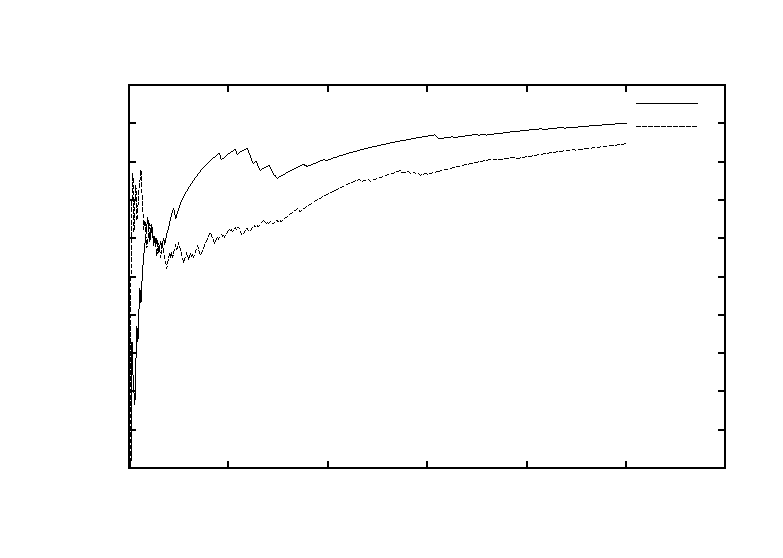
\includegraphics[width=0.5\textwidth]{plots/tiger}
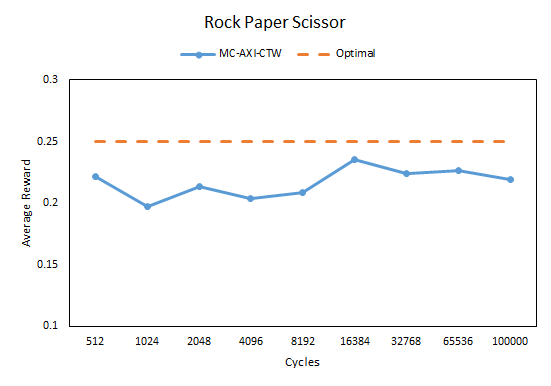
\includegraphics[width=0.5\textwidth]{plots/rps}
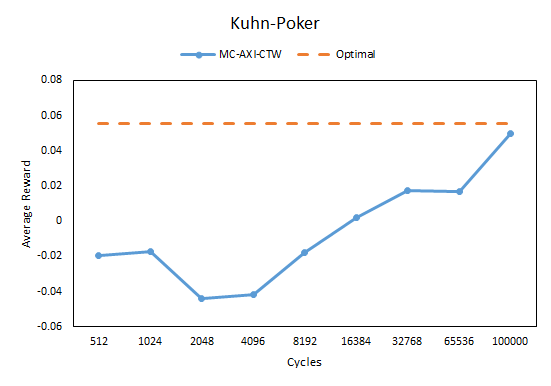
\includegraphics[width=0.5\textwidth]{plots/kpok}
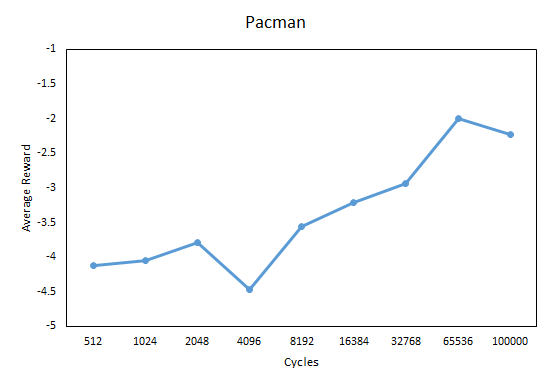
\includegraphics[width=0.5\textwidth]{plots/pacman}
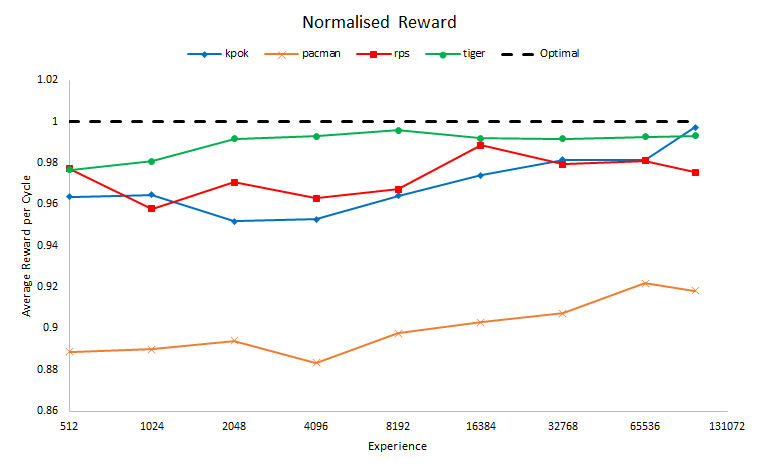
\includegraphics[width=\textwidth]{plots/normalised}
%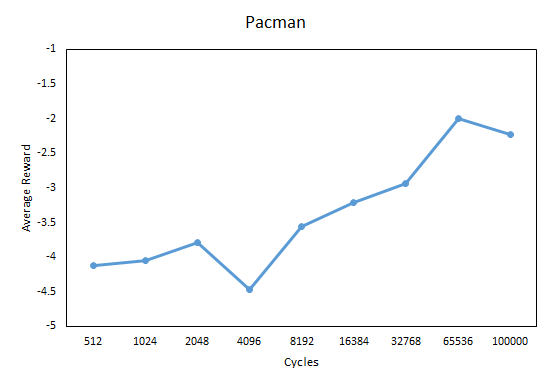
\includegraphics[width=386px]{plots/pacman}
\caption{\label{plot:rewards}Average Reward per Cycle vs Experience}
\end{figure}

\setlength\parindent{0pt}

\pagebreak
\subsection{Further Experiments}

\paragraph{0.2 Coin vs 0.8 Coin} To see how well the agent handles a sudden change of the environment, we conducted the following experiment. The agent is trained in a simple 0.8 biased coinflip environment and the generated context tree is saved. This data is then loaded in a new 0.2 biased coinflip environment. The agent was evaluated during 20000 cycles with the following settings:

\bigskip

\begin{tabular}{|l|c|c|c|c|c|}
\hline
Domain & CTW depth & $m$ & $\epsilon$ & $\rho$UCT Simulations & bias $p$\\\hline
Coinflip A & 16 & 2 & 0.999 & 100 & 0.8\\
Coinflip B & 16 & 2 & 0.999 & 100 & 0.2\\\hline
\end{tabular}

\bigskip

These values were chosen to give reasonable speed and accuracy. In detail, the following experiments were conducted:

\begin{enumerate}
 \setlength{\itemsep}{0cm}%
  \setlength{\parskip}{0cm}%
\item environment A with exploration=0.2,\emph{ save context tree}\label{coinflip_a_ct}
\item environment A with exploration=0
\item environment A with exploration=0, \emph{context tree A loaded}
\item environment B, exploration = 0.2 (expected: same result as in 1.)
\item environment B, exploration = 0 (expected: same result as in 2.)
\item environment B with exploration = 0, \emph{context tree A loaded}
\item environment B with exploration = 0.2, \emph{context tree A loaded}
\end{enumerate}

Experiments 1-5 should be seen as reference values for the settings in 6-7 where the agent acts in environment B with the model of environment A. The most interesting results are summarized in figure \ref{plot:cointests}.  Compared to the normal learning case (4) the agent does not perform well anymore in the new environment if exploration is suppressed (6) and it only slowly learns the new strategy. If exploration is permitted the new environment can be learned faster (7). To reach a 0.75 average reward it took the agent 1600 cycles in setting (4), 10700 cycles in setting (6) and 5000 cycles in setting (7). Full results are presented in figure \ref{plot:cointests_all}.

\paragraph{Biased RPS vs Tiger}
A similar experiment was also conducted on the biased rock-paper-scissor and tiger domains. The agent was evaluated during 20000 cycles with the following settings:

\bigskip

\begin{tabular}{|l|c|c|c|c|c|}
\hline
Domain & CTW depth & $m$ & $\epsilon$ &$\gamma $ & $\rho$ UCT Simulations\\\hline
Tiger & 32 & 5 & 0.999 & 0.99 & 500\\
rps & 32 & 5 & 0.999 & 0.99 & 500\\\hline
\end{tabular}

\bigskip

The following test runs where recorded:
\begin{enumerate}
 \setlength{\itemsep}{0cm}%
  \setlength{\parskip}{0cm}%
\item tiger environment,\emph{ save context tree}
\item tiger environment with exploration=0, context tree loaded
\item rock-paper-scissor environment
\item rock-paper-scissor environment with exploration=0
\item rock-paper-scissor environment, \emph{tiger context tree loaded} 
\item rock-paper-scissor environment with exploration=0, \emph{tiger context tree loaded} 
\end{enumerate}

The results for (3), (5), (6) are presented in figure \ref{plot:cointests}. In this case the context tree structure from a different environment doesn't seem to affect the agent. Moreover, with exploration turned off the agent performs better in spite of the `wrong' model. To explain this we have to assume that the context tree of the tiger environment is similar to the one generated in rock-paper-scissor, so forgetting old percepts is not necessary. Results of all test runs can be found in figure \ref{plot:cointests_all}.

\begin{figure}[h]
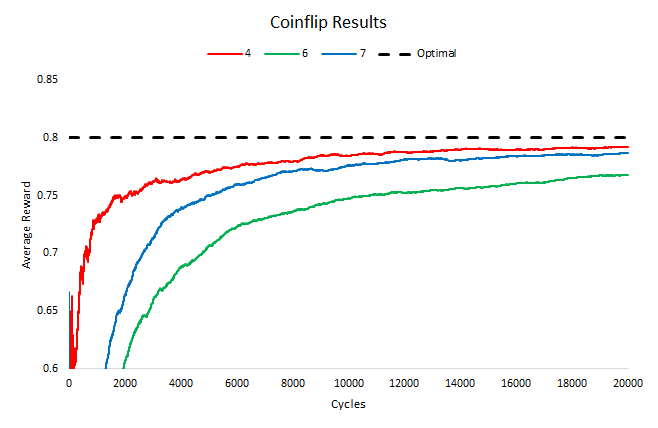
\includegraphics[width=0.5\textwidth]{plots/coinflip_tests1}
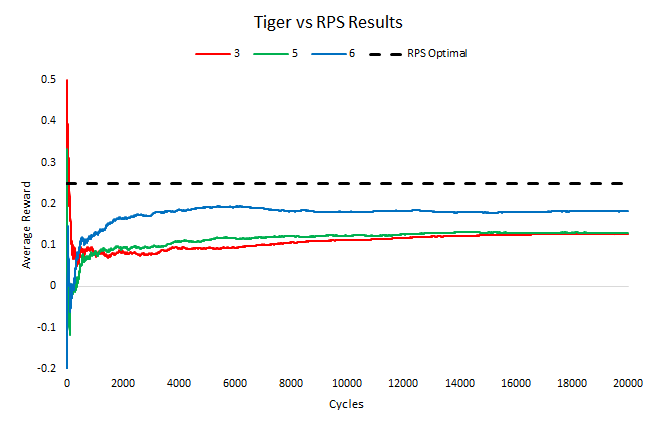
\includegraphics[width=0.5\textwidth]{plots/rps_tiger_1}
\caption{\label{plot:cointests}Further experiments}
\end{figure}

\begin{figure}[h]
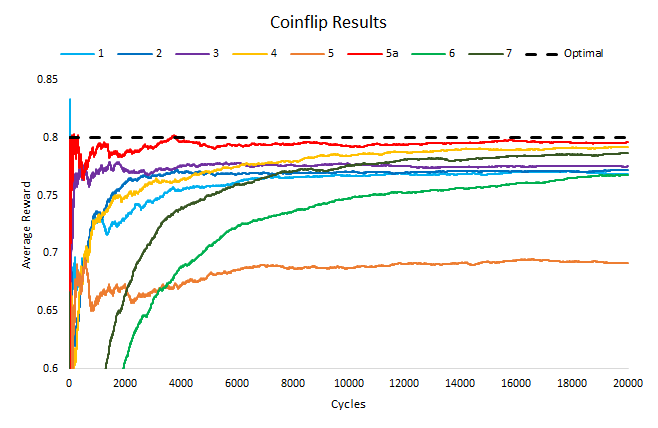
\includegraphics[width=0.5\textwidth]{plots/coinflip_tests}
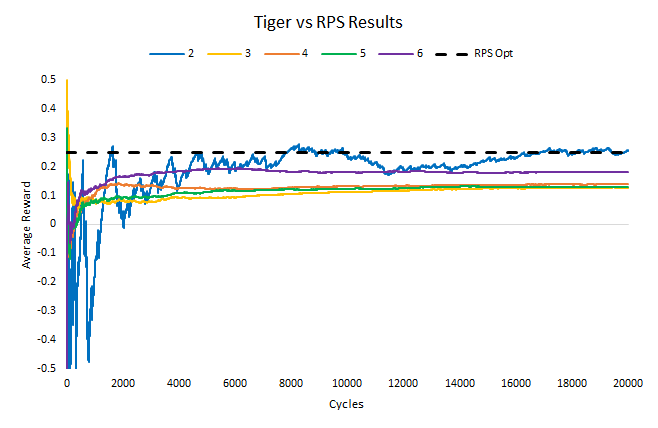
\includegraphics[width=0.5\textwidth]{plots/rps_tiger_trim}
\caption{\label{plot:cointests_all}Further experiments, all results. Result (5) in the coinflip experiment seems to be an outlier, the agent was run again with the same settings resulting in (5a). The reason for this is probably the use of a single context tree instead of a factored context tree.}
\end{figure}

%sample graph
%\begin{figure}
%% GNUPLOT: LaTeX picture with Postscript
\begingroup
  \makeatletter
  \providecommand\color[2][]{%
    \GenericError{(gnuplot) \space\space\space\@spaces}{%
      Package color not loaded in conjunction with
      terminal option `colourtext'%
    }{See the gnuplot documentation for explanation.%
    }{Either use 'blacktext' in gnuplot or load the package
      color.sty in LaTeX.}%
    \renewcommand\color[2][]{}%
  }%
  \providecommand\includegraphics[2][]{%
    \GenericError{(gnuplot) \space\space\space\@spaces}{%
      Package graphicx or graphics not loaded%
    }{See the gnuplot documentation for explanation.%
    }{The gnuplot epslatex terminal needs graphicx.sty or graphics.sty.}%
    \renewcommand\includegraphics[2][]{}%
  }%
  \providecommand\rotatebox[2]{#2}%
  \@ifundefined{ifGPcolor}{%
    \newif\ifGPcolor
    \GPcolorfalse
  }{}%
  \@ifundefined{ifGPblacktext}{%
    \newif\ifGPblacktext
    \GPblacktexttrue
  }{}%
  % define a \g@addto@macro without @ in the name:
  \let\gplgaddtomacro\g@addto@macro
  % define empty templates for all commands taking text:
  \gdef\gplbacktext{}%
  \gdef\gplfronttext{}%
  \makeatother
  \ifGPblacktext
    % no textcolor at all
    \def\colorrgb#1{}%
    \def\colorgray#1{}%
  \else
    % gray or color?
    \ifGPcolor
      \def\colorrgb#1{\color[rgb]{#1}}%
      \def\colorgray#1{\color[gray]{#1}}%
      \expandafter\def\csname LTw\endcsname{\color{white}}%
      \expandafter\def\csname LTb\endcsname{\color{black}}%
      \expandafter\def\csname LTa\endcsname{\color{black}}%
      \expandafter\def\csname LT0\endcsname{\color[rgb]{1,0,0}}%
      \expandafter\def\csname LT1\endcsname{\color[rgb]{0,1,0}}%
      \expandafter\def\csname LT2\endcsname{\color[rgb]{0,0,1}}%
      \expandafter\def\csname LT3\endcsname{\color[rgb]{1,0,1}}%
      \expandafter\def\csname LT4\endcsname{\color[rgb]{0,1,1}}%
      \expandafter\def\csname LT5\endcsname{\color[rgb]{1,1,0}}%
      \expandafter\def\csname LT6\endcsname{\color[rgb]{0,0,0}}%
      \expandafter\def\csname LT7\endcsname{\color[rgb]{1,0.3,0}}%
      \expandafter\def\csname LT8\endcsname{\color[rgb]{0.5,0.5,0.5}}%
    \else
      % gray
      \def\colorrgb#1{\color{black}}%
      \def\colorgray#1{\color[gray]{#1}}%
      \expandafter\def\csname LTw\endcsname{\color{white}}%
      \expandafter\def\csname LTb\endcsname{\color{black}}%
      \expandafter\def\csname LTa\endcsname{\color{black}}%
      \expandafter\def\csname LT0\endcsname{\color{black}}%
      \expandafter\def\csname LT1\endcsname{\color{black}}%
      \expandafter\def\csname LT2\endcsname{\color{black}}%
      \expandafter\def\csname LT3\endcsname{\color{black}}%
      \expandafter\def\csname LT4\endcsname{\color{black}}%
      \expandafter\def\csname LT5\endcsname{\color{black}}%
      \expandafter\def\csname LT6\endcsname{\color{black}}%
      \expandafter\def\csname LT7\endcsname{\color{black}}%
      \expandafter\def\csname LT8\endcsname{\color{black}}%
    \fi
  \fi
  \setlength{\unitlength}{0.0500bp}%
  \begin{picture}(7200.00,5040.00)%
    \gplgaddtomacro\gplbacktext{%
      \csname LTb\endcsname%
      \put(946,704){\makebox(0,0)[r]{\strut{} 0}}%
      \put(946,1156){\makebox(0,0)[r]{\strut{} 0.1}}%
      \put(946,1609){\makebox(0,0)[r]{\strut{} 0.2}}%
      \put(946,2061){\makebox(0,0)[r]{\strut{} 0.3}}%
      \put(946,2513){\makebox(0,0)[r]{\strut{} 0.4}}%
      \put(946,2966){\makebox(0,0)[r]{\strut{} 0.5}}%
      \put(946,3418){\makebox(0,0)[r]{\strut{} 0.6}}%
      \put(946,3870){\makebox(0,0)[r]{\strut{} 0.7}}%
      \put(946,4323){\makebox(0,0)[r]{\strut{} 0.8}}%
      \put(946,4775){\makebox(0,0)[r]{\strut{} 0.9}}%
      \put(1078,484){\makebox(0,0){\strut{} 0}}%
      \put(2223,484){\makebox(0,0){\strut{} 2000}}%
      \put(3368,484){\makebox(0,0){\strut{} 4000}}%
      \put(4513,484){\makebox(0,0){\strut{} 6000}}%
      \put(5658,484){\makebox(0,0){\strut{} 8000}}%
      \put(6803,484){\makebox(0,0){\strut{} 10000}}%
      \put(176,2739){\rotatebox{-270}{\makebox(0,0){\strut{}average reward}}}%
      \put(3940,154){\makebox(0,0){\strut{}cycle}}%
    }%
    \gplgaddtomacro\gplfronttext{%
      \csname LTb\endcsname%
      \put(5816,4602){\makebox(0,0)[r]{\strut{}coinflip first run}}%
      \csname LTb\endcsname%
      \put(5816,4382){\makebox(0,0)[r]{\strut{}pretrained ct, no exploration}}%
      \csname LTb\endcsname%
      \put(5816,4162){\makebox(0,0)[r]{\strut{}optimal}}%
    }%
    \gplbacktext
    \put(0,0){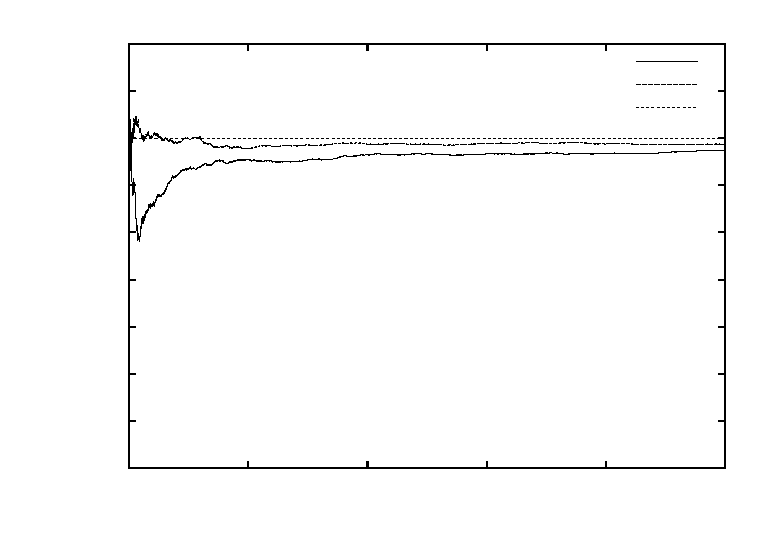
\includegraphics{plots/coinflip}}%
    \gplfronttext
  \end{picture}%
\endgroup

%\caption{\label{plot:coinflip}Results on the coinflip environment}
%\end{figure}


%\subsection{Discussion}
%
%Include statistics about cycles required for optimal performance, time per cycle as in the VNHS paper \cite{VNHS09}. Also note the number of simulations required at each cycle for near optimal performance.
\newpage
\bibliographystyle{alpha}
\bibliography{references}

\end{document}
